\documentclass[journal,12pt,twocolumn]{IEEEtran}
%
\usepackage{setspace}
\usepackage{gensymb}
\usepackage{siunitx}
\usepackage{tkz-euclide} 
\usepackage{textcomp}
\usepackage{standalone}
\usetikzlibrary{calc}
\newcommand\hmmax{0}
\newcommand\bmmax{0}

%\doublespacing
\singlespacing

%\usepackage{graphicx}
%\usepackage{amssymb}
%\usepackage{relsize}
\usepackage[cmex10]{amsmath}
%\usepackage{amsthm}
%\interdisplaylinepenalty=2500
%\savesymbol{iint}
%\usepackage{txfonts}
%\restoresymbol{TXF}{iint}
%\usepackage{wasysym}
\usepackage{amsthm}
%\usepackage{iithtlc}
\usepackage{mathrsfs}
\usepackage{txfonts}
\usepackage{stfloats}
\usepackage{bm}
\usepackage{cite}
\usepackage{cases}
\usepackage{subfig}
%\usepackage{xtab}
\usepackage{longtable}
\usepackage{multirow}
%\usepackage{algorithm}
%\usepackage{algpseudocode}
\usepackage{enumitem}
\usepackage{mathtools}
\usepackage{steinmetz}
\usepackage{tikz}
\usepackage{circuitikz}
\usepackage{verbatim}
\usepackage{tfrupee}
\usepackage[breaklinks=true]{hyperref}
%\usepackage{stmaryrd}
\usepackage{tkz-euclide} % loads  TikZ and tkz-base
%\usetkzobj{all}
\usetikzlibrary{calc,math}
\usepackage{listings}
    \usepackage{color}                                            %%
    \usepackage{array}                                            %%
    \usepackage{longtable}                                        %%
    \usepackage{calc}                                             %%
    \usepackage{multirow}                                         %%
    \usepackage{hhline}                                           %%
    \usepackage{ifthen}                                           %%
  %optionally (for landscape tables embedded in another document): %%
    \usepackage{lscape}     
\usepackage{multicol}
\usepackage{chngcntr}
\usepackage{amsmath}
\usepackage{cleveref}
%\usepackage{enumerate}

%\usepackage{wasysym}
%\newcounter{MYtempeqncnt}
\DeclareMathOperator*{\Res}{Res}
%\renewcommand{\baselinestretch}{2}
\renewcommand\thesection{\arabic{section}}
\renewcommand\thesubsection{\thesection.\arabic{subsection}}
\renewcommand\thesubsubsection{\thesubsection.\arabic{subsubsection}}

\renewcommand\thesectiondis{\arabic{section}}
\renewcommand\thesubsectiondis{\thesectiondis.\arabic{subsection}}
\renewcommand\thesubsubsectiondis{\thesubsectiondis.\arabic{subsubsection}}

% correct bad hyphenation here
\hyphenation{op-tical net-works semi-conduc-tor}
\def\inputGnumericTable{}                                 %%

\lstset{
%language=C,
frame=single, 
breaklines=true,
columns=fullflexible
}
%\lstset{
%language=tex,
%frame=single, 
%breaklines=true
%}
\usepackage{graphicx}
\usepackage{pgfplots}

\begin{document}


\newtheorem{theorem}{Theorem}[section]
\newtheorem{problem}{Problem}
\newtheorem{proposition}{Proposition}[section]
\newtheorem{lemma}{Lemma}[section]
\newtheorem{corollary}[theorem]{Corollary}
\newtheorem{example}{Example}[section]
\newtheorem{definition}[problem]{Definition}
%\newtheorem{thm}{Theorem}[section] 
%\newtheorem{defn}[thm]{Definition}
%\newtheorem{algorithm}{Algorithm}[section]
%\newtheorem{cor}{Corollary}
\newcommand{\BEQA}{\begin{eqnarray}}
\newcommand{\EEQA}{\end{eqnarray}}
\newcommand{\define}{\stackrel{\triangle}{=}}
\bibliographystyle{IEEEtran}
%\bibliographystyle{ieeetr}
\providecommand{\mbf}{\mathbf}
\providecommand{\abs}[1]{\ensuremath{\left\vert#1\right\vert}}
\providecommand{\norm}[1]{\ensuremath{\left\lVert#1\right\rVert}}
\providecommand{\mean}[1]{\ensuremath{E\left[ #1 \right]}}
\providecommand{\pr}[1]{\ensuremath{\Pr\left(#1\right)}}
\providecommand{\qfunc}[1]{\ensuremath{Q\left(#1\right)}}
\providecommand{\sbrak}[1]{\ensuremath{{}\left[#1\right]}}
\providecommand{\lsbrak}[1]{\ensuremath{{}\left[#1\right.}}
\providecommand{\rsbrak}[1]{\ensuremath{{}\left.#1\right]}}
\providecommand{\brak}[1]{\ensuremath{\left(#1\right)}}
\providecommand{\lbrak}[1]{\ensuremath{\left(#1\right.}}
\providecommand{\rbrak}[1]{\ensuremath{\left.#1\right)}}
\providecommand{\cbrak}[1]{\ensuremath{\left\{#1\right\}}}
\providecommand{\lcbrak}[1]{\ensuremath{\left\{#1\right.}}
\providecommand{\rcbrak}[1]{\ensuremath{\left.#1\right\}}}
\theoremstyle{remark}
\newtheorem{rem}{Remark}
\newcommand{\sgn}{\mathop{\mathrm{sgn}}}
\providecommand{\res}[1]{\Res\displaylimits_{#1}} 
%\providecommand{\norm}[1]{\lVert#1\rVert}
\providecommand{\mtx}[1]{\mathbf{#1}}
\providecommand{\fourier}{\overset{\mathcal{F}}{ \rightleftharpoons}}
%\providecommand{\hilbert}{\overset{\mathcal{H}}{ \rightleftharpoons}}
\providecommand{\system}{\overset{\mathcal{H}}{ \longleftrightarrow}}
	%\newcommand{\solution}[2]{\textbf{Solution:}{#1}}
\newcommand{\solution}{\noindent \textbf{Solution: }}
\newcommand{\cosec}{\,\text{cosec}\,}
\providecommand{\dec}[2]{\ensuremath{\overset{#1}{\underset{#2}{\gtrless}}}}
\newcommand{\myvec}[1]{\ensuremath{\begin{pmatrix}#1\end{pmatrix}}}
\newcommand{\mydet}[1]{\ensuremath{\begin{vmatrix}#1\end{vmatrix}}}
%\numberwithin{equation}{section}
\numberwithin{equation}{subsection}
%\numberwithin{problem}{section}
%\numberwithin{definition}{section}
\makeatletter
\@addtoreset{figure}{problem}
\makeatother
\let\StandardTheFigure\thefigure
\let\vec\mathbf
%\renewcommand{\thefigure}{\theproblem.\arabic{figure}}
\renewcommand{\thefigure}{\theproblem}
%\setlist[enumerate,1]{before=\renewcommand\theequation{\theenumi.\arabic{equation}}
%\counterwithin{equation}{enumi}
%\renewcommand{\theequation}{\arabic{subsection}.\arabic{equation}}
\def\putbox#1#2#3{\makebox[0in][l]{\makebox[#1][l]{}\raisebox{\baselineskip}[0in][0in]{\raisebox{#2}[0in][0in]{#3}}}}
     \def\rightbox#1{\makebox[0in][r]{#1}}
     \def\centbox#1{\makebox[0in]{#1}}
     \def\topbox#1{\raisebox{-\baselineskip}[0in][0in]{#1}}
     
 \vspace{3cm}
 \title{Assignment 6}
 \author{Matish Singh Tanwar}
 \maketitle
 \newpage
 \bigskip
 %\renewcommand{\thefigure}{\theenumi}
 \renewcommand{\thetable}{\theenumi}
\vspace{1.0cm}
\begin{abstract}
This document solves question based on affine transformation.
\end{abstract}
\vspace{0.5cm}
%
Download all python codes from 
\begin{lstlisting}
https://github.com/Matish007/Matrix-Theory-EE5609-/tree/master/Assignment_6/Codes
\end{lstlisting}
%
and latex-tikz codes from 
\begin{lstlisting}
https://github.com/Matish007/Matrix-Theory-EE5609-/tree/master/Assignment_6
\end{lstlisting}
%
%
\vspace{0.5mm}
\section{Problem}
Show that,by rotating axes,the equation
\begin{align}
 \vec{x}^T\myvec{41&12\\12&34}\vec{x}=75\label{1}
\end{align}
can be reduced to
\begin{align}
 \vec{x}^T\myvec{2&0\\0&1}\vec{x}=3
\end{align}
%
\section {Explanation}
The given equation is of the form
\begin{align}
   \vec{x}^T\vec{V}\vec{x}+f=0\\
   f=-75
\end{align}
The matrix $\vec{V}$ can be decomposed as
\begin{align}
    \vec{V}=\vec{P}\vec{D}\vec{P}^T\label{2}\\
    \text{where  }\vec{D}=\myvec{\lambda_1&0\\0&\lambda_2}
\end{align}
$\lambda_1$ and $\lambda_2$ are eigen values of $\vec{V}$  and
$\vec{P}$ contains the eigen vectors corresponding to the eigen values $\lambda_1$ and $\lambda_2$
\begin{align}
\vec{x}=\vec{P}\vec{y}+\vec{c}
\end{align}
indicates the linear transformation where $\vec{P}$ indicates the rotation of axes and $\vec{c}$ gives the shift of origin.
\begin{align}
  \vec{V}=\myvec{41&12\\12&34}\\
  det(\vec{V} )=\mydet{41&12\\12&34}>0
\end{align}
So,the given equation represents an ellipse\\
To find the Eigen values of $\vec{V}$
\begin{align}
    \mydet{\lambda\vec{I}-\vec{v}}=0\\
    \implies \mydet{\lambda-41&-12\\-12&\lambda-34}=0\\
    \implies \lambda^2-75\lambda+1250=0\\
    \implies \lambda_1=50,\lambda_2=25\\
    \vec{D}=\myvec{50&0\\0&25}
\end{align}
Finding Eigen vector $\vec{p}_1$ ,
\begin{align}
\lambda_1\vec{I}-\vec{V}= \myvec{9&-12\\-12&16}\xleftrightarrow[R_2\leftarrow R_2/4]{R_1\leftarrow R_1/3}\myvec{3&-4\\-3&4}\\
\xleftrightarrow[]{R_2\leftarrow R_1+R_2}\myvec{3&-4\\0&0}\\
\implies \vec{p_1}=\frac{1}{\sqrt{4^2+3^2}}\myvec{4\\3}=\myvec{\frac{4}{5}\\\frac{3}{5}}
\end{align}
Similarly,
\begin{align}
  \lambda_2\vec{I}-\vec{V}= \myvec{-16&-12\\-12&-9}\xleftrightarrow[R_2\leftarrow R_2/-3]{R_1\leftarrow R_1/-4}\myvec{4&3\\4&3}\\
\xleftrightarrow[]{R_2\leftarrow R_1-R_2}\myvec{4&3\\0&0}\\
\implies \vec{p_2}=\frac{1}{\sqrt{4^2+3^2}}\myvec{-3\\4}=\myvec{\frac{-3}{5}\\\frac{4}{5}}\\\text{ Therefore, } \vec{P}=\myvec{\vec{p_1}&\vec{p_2}}=\myvec{\frac{4}{5}&\frac{-3}{5}\\ \frac{3}{5}&\frac{4}{5}}
\end{align}
From \eqref{2} $\vec{V}$ can be rewritten as
\begin{align}
    \vec{V}=\myvec{\frac{4}{5}&\frac{-3}{5}\\ \frac{3}{5}&\frac{4}{5}}\myvec{50&0\\0&25}\myvec{\frac{4}{5}&\frac{3}{5}\\ \frac{-3}{5}&\frac{4}{5}}
\end{align}
\eqref{1} can be now rewritten as
\begin{align}
25\left[\vec{x}^T\myvec{\frac{4}{5}&\frac{-3}{5}\\ \frac{3}{5}&\frac{4}{5}}\myvec{2&0\\0&1}\myvec{\frac{4}{5}&\frac{3}{5}\\ \frac{-3}{5}&\frac{4}{5}}\vec{x}\right]=75\\
  \left[\myvec{\frac{4}{5}&\frac{3}{5}\\ \frac{-3}{5}&\frac{4}{5}}\vec{x}\right]^T\myvec{2&0\\0&1}\left[\myvec{\frac{4}{5}&\frac{3}{5}\\ \frac{-3}{5}&\frac{4}{5}}\vec{x}\right]= 3\label{3}
\end{align}
 Consider the rotation transformation 
\begin{align}
  \vec{x}=\vec{P}\vec{y}\\
  \implies \vec{x}=\myvec{\frac{4}{5}&\frac{-3}{5}\\ \frac{3}{5}&\frac{4}{5}}\vec{y}\label{4}\\
  \vec{P}^{-1}\vec{x}=\vec{P}^{-1}\vec{P}\vec{y}\\
  \implies \vec{y}= \vec{P}^{-1}\vec{x}\\
  \text{But, }\vec{P}^{-1}=\vec{P}^T\\
  \implies \vec{y}=\myvec{\frac{4}{5}&\frac{3}{5}\\ \frac{-3}{5}&\frac{4}{5}}\vec{x}
\end{align}
Using \eqref{4} in \eqref{3}, the ellipse equation can be rewritten as
\begin{align}
     \vec{y}^T\myvec{2&0\\0&1}\vec{y}=3
\end{align}
\begin{figure}[!ht]
\centering
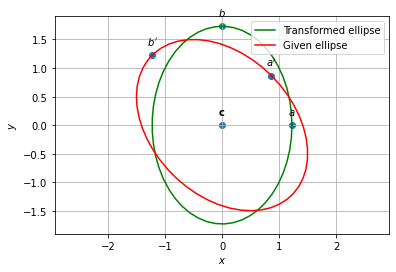
\includegraphics[width=\columnwidth]{ellipse.png}
\caption{plot showing the original and rotated ellipse}
\label{Fig}
\end{figure}
\end{document}